
\section{Calibrazione dei rivelatori}
I rivelatori di quasi picco e media devono essere necessariamente calibrati
secondo i valori e le metodologie fornite dalla norma.
La prima metodologia di calibrazione analizzata viene chiamata \textbf{assoluta} (in ampiezza), 
si definisce l'area \textit{IS} dell'impulso con la seguente:
$$
IS = \int_{-\infty}^{+\infty} v(t) dt
$$

Riferendosi alla tabella sottostante, la calibrazione del rivelatore di quasi-picco
viene effettuata mediante l'analisi della risposta agli impulsi con area
\textit{IS} pari ad \textit{a)}, spettro uniforme almeno fino a \textit{b)}, e
frequenza di ripetizione pari a \textit{c)}, deve essere la stessa (entro \SI{1.5}{\decibel}) di un
segnale sinusoidale non modulato di pari frequenza, avente un'ampiezza
di valore efficace pari a \SI{2}{\milli\volt} ossia \SI{66}{\decibel\micro\volt}.
\begin{center} %tabella parametri calibrazione assoluta
 \begin{tabular}{|>{\centering}p{4cm}|>{\centering}p{2.8cm}|>{\centering}p{2.8cm}|p{2.8cm}<{\centering}|}
  \hline
    \textbf{Frequency range} & \textbf{a)} \si{\micro\volt\second} & \textbf{b)} \si{\mega\hertz} & \textbf{c)} \si{\hertz} \\ \hline
    \SI{9}{\kilo\hertz} to \SI{150}{\kilo\hertz}     & 13.5  & 0.15 & 25  \\ \hline
    \SI{150}{\kilo\hertz} to \SI{30}{\mega\hertz}    & 0.316 & 30   & 100 \\ \hline
    \SI{30}{\mega\hertz} to \SI{300}{\mega\hertz}    & 0.044 & 300  & 100 \\ \hline
    \SI{300}{\mega\hertz} to \SI{1000}{\mega\hertz}  & 0.044 & 1000 & 100 \\ \hline
 \end{tabular}
\end{center}

Si analizza ora la calibrazione \textbf{relativa} (in frequenza).
Seguendo la curva in figura \ref{fig:calibrazione_relativa} si valuta 
la variazione di \textit{ampiezza} da dare al segale al variare
della frequenza di ripetizione per ottenere sempre la stessa
indicazione di quasi-picco dallo strumento.

\begin{figure}[h] %figura calibrazione relativa
 \centering
 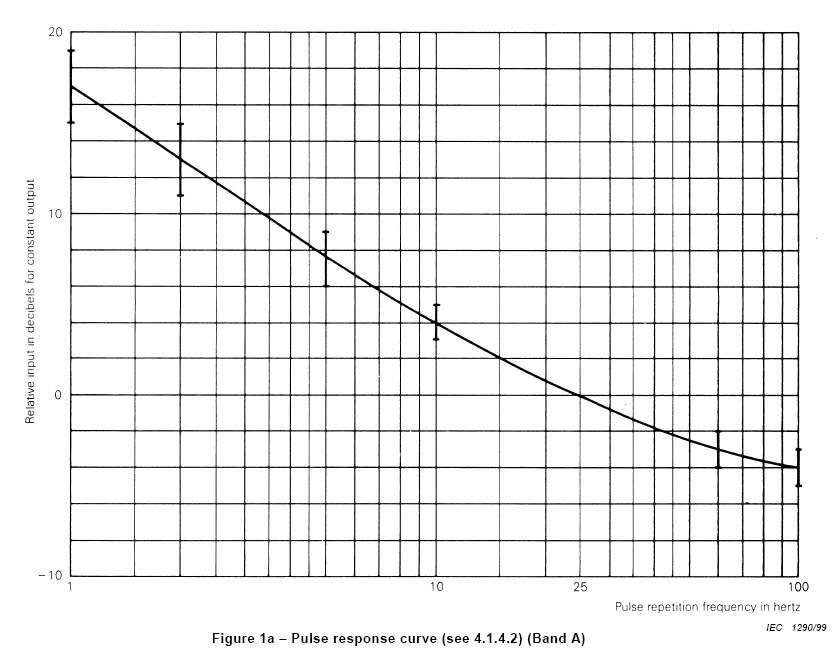
\includegraphics[width=0.7\textwidth]{calibrazione_relativa}
 \caption{Valore del segnale da fornire al variare della frequenza di ripetizione}
 \label{fig:calibrazione_relativa}
\end{figure}


